\begin{landscape}
\begin{figure}[!]
    \centering
    \captionlistentry{Level Scheme of $^{156}$Gd. The gamma ray of the $4^+_{gs}\rightarrow 2^+_{gs}$ (199 keV) transition in the ground state was gated on. It was then compared with the gated spectrum from the gamma ray of the $6^+_{gs}\rightarrow 4^+_{gs}$ (296 keV) transition in the ground state. Peaks only appearing in the first gate were assumed to go into the $4^+_{gs}$ state, and assignments were made. Additionally, these peaks were also gated on, to look for cascades leading into the $4^+_{gs}$ state, which were found in several cases. The levels are organized by band. The lower levels of the band, unseen by gamma rays in this gate, are in blue.}
    \label{fig:156_4to2}
    \begin{subfigure}{1.4\textwidth}
    \caption*{\centering \fontsize{10pt}{12pt}Figure \ref{fig:156_4to2}. Level Scheme of $^{156}$Gd. The gamma ray of the $4^+_{gs}\rightarrow 2^+_{gs}$ (199 keV) transition in the ground state was gated on. It was then compared with the gated spectrum from the gamma ray of the $6^+_{gs}\rightarrow 4^+_{gs}$ (296 keV) transition in the ground state. Peaks only appearing in the first gate were assumed to go into the $4^+_{gs}$ state, and assignments were made. Additionally, these peaks were also gated on, to look for cascades leading into the $4^+_{gs}$ state, which were found in several cases. The levels are organized by band. The lower levels of the band, unseen by gamma rays in this gate, are in blue.}
    \end{subfigure}
\end{figure}
\clearpage
\begin{figure}
    \ContinuedFloat
    \begin{subfigure}{1.4\textwidth}
    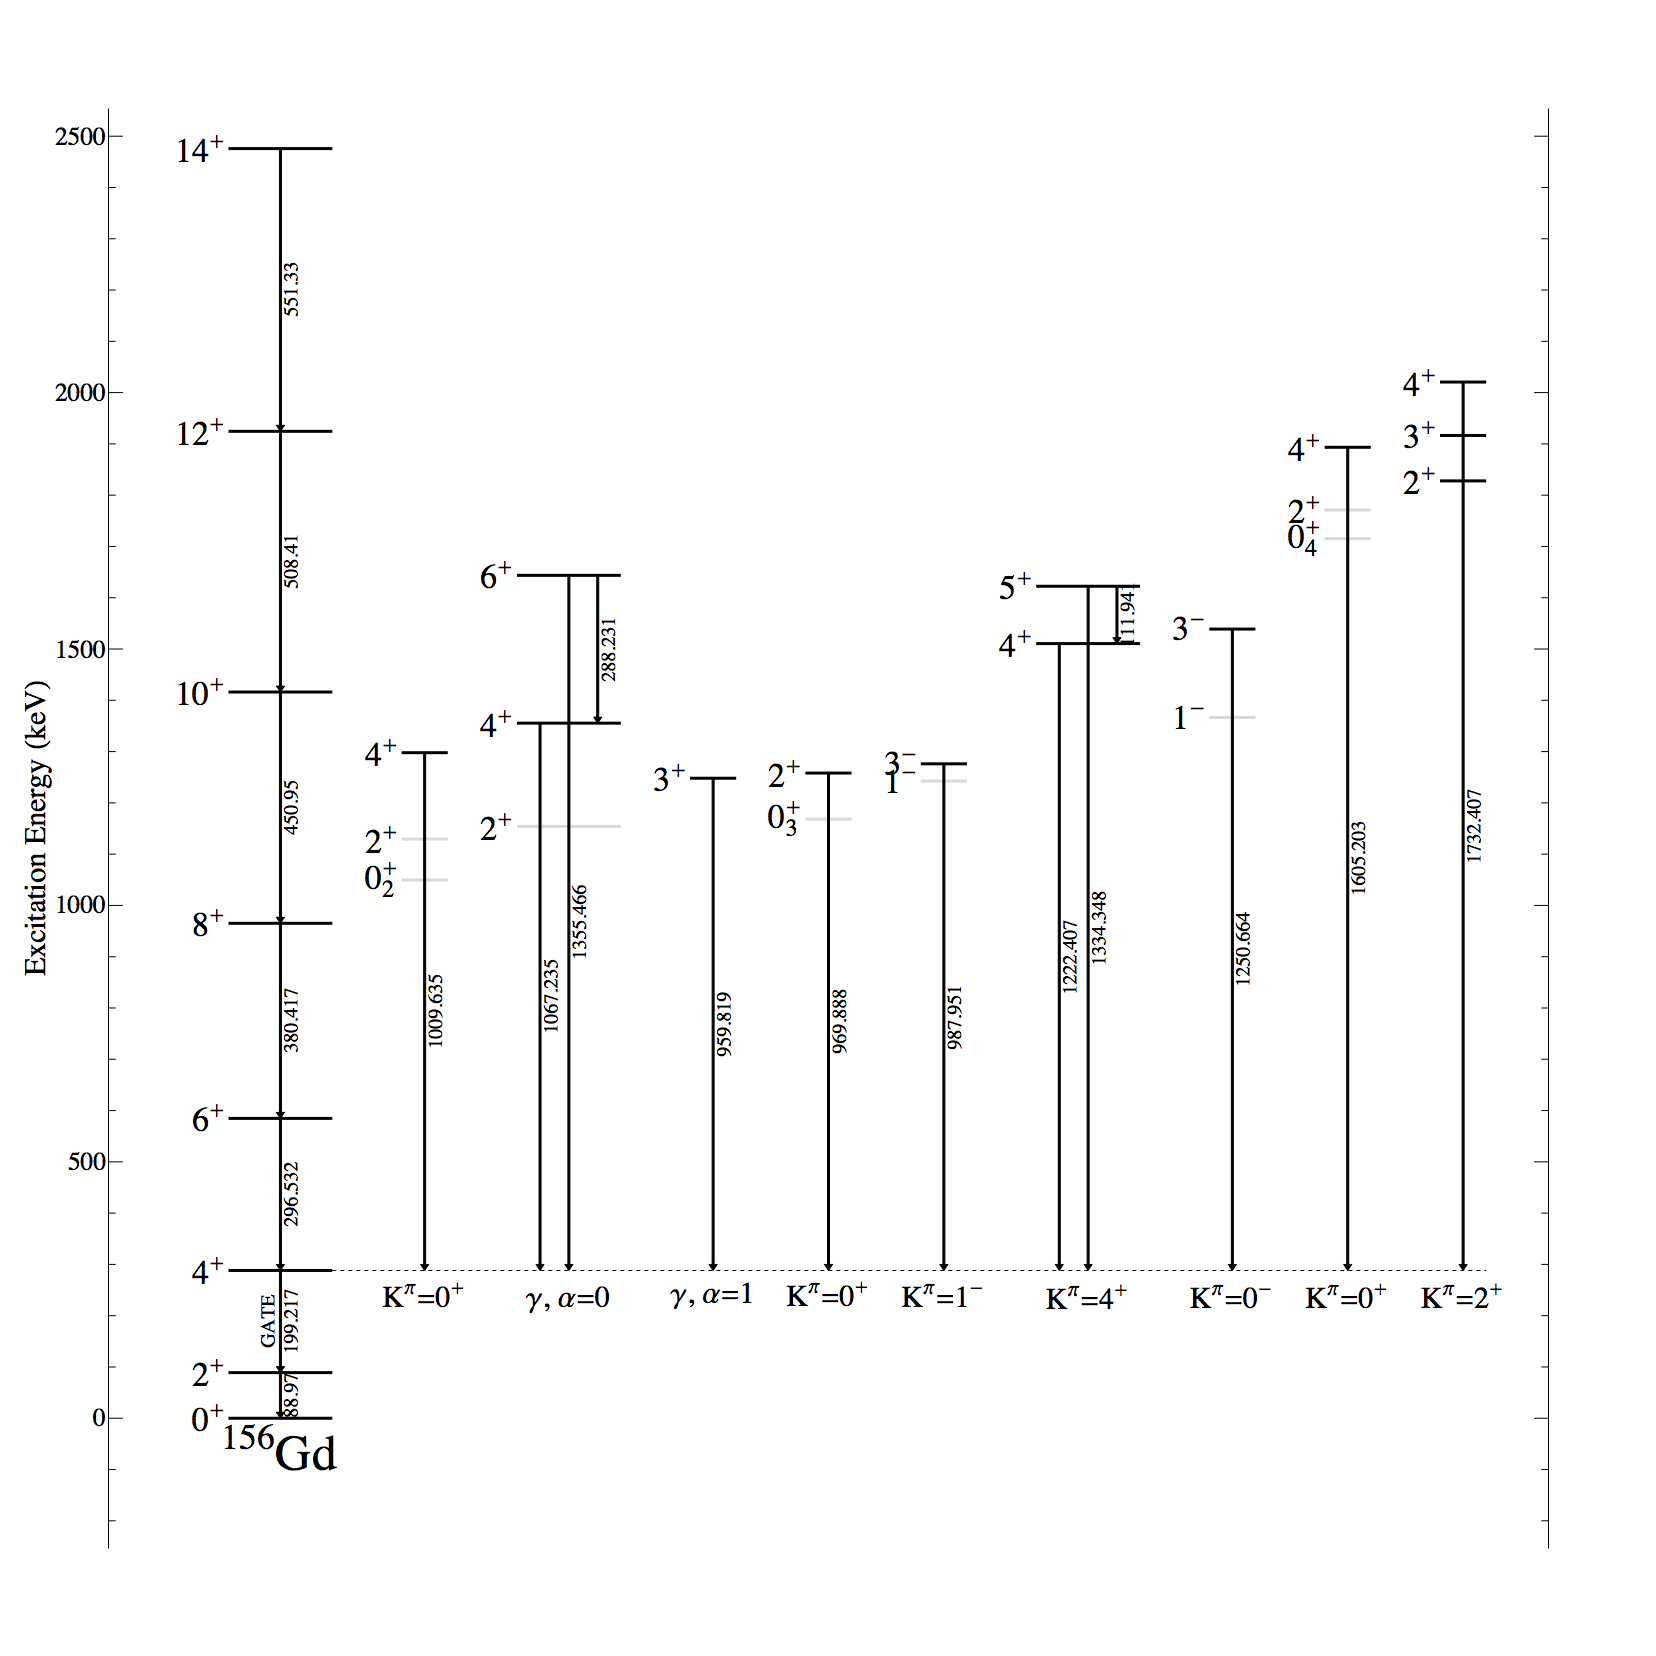
\includegraphics[scale=0.33]{156GdTablesAndFigs/156Gd_4to2.eps}
    \label{fig:156_4to2level}
    \end{subfigure}
\end{figure}
\end{landscape}
\begin{figure}
    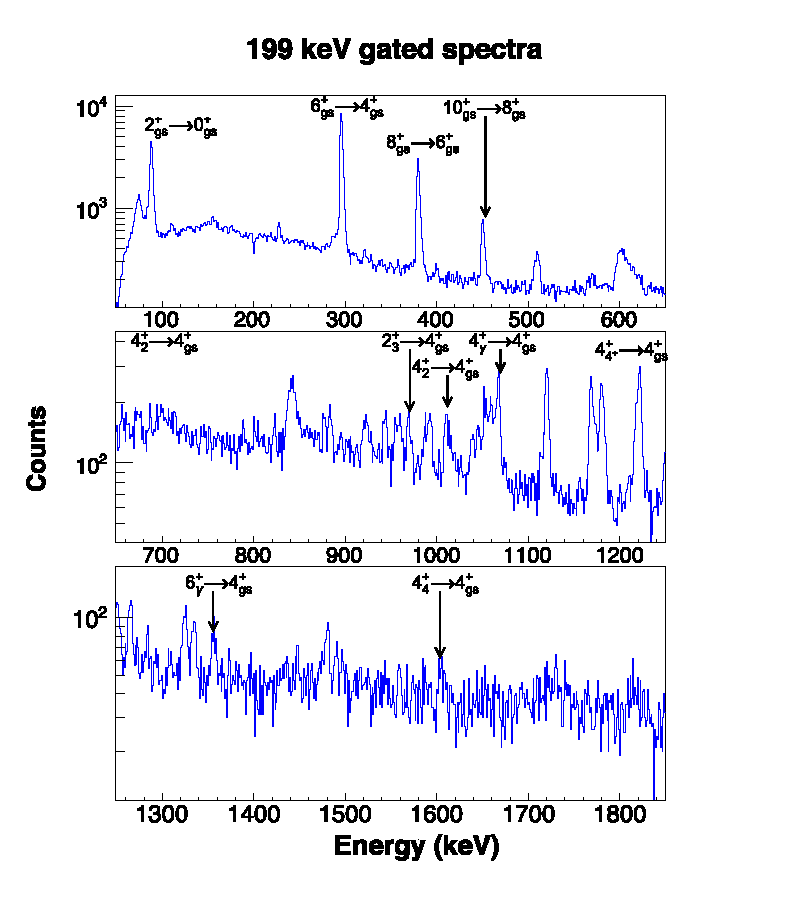
\includegraphics[scale=1.3]{156GdTablesAndFigs/199_gamma.eps}
    \caption{Gamma spectrum gated on 199 keV, corresponding to the $4^+_{gs}\rightarrow 2^+_{gs}$ transition. Several transitions are marked according to the level scheme in Figure \ref{fig:156_4to2}.}
    \label{fig:156_4to2spec}
\end{figure}